\documentclass[letterpaper,11pt]{article}
\usepackage{graphicx}
\usepackage{listings}
\usepackage{hyperref}
\usepackage{amsmath}
\usepackage{url}
\def\UrlBreaks{\do\/\do-}
\usepackage[normalem]{ulem}
\newcommand{\tab}[1]{\hspace{.2\textwidth}\rlap{#1}}
\usepackage{float}
\restylefloat{table}
\usepackage{xcolor}
\usepackage{sectsty}
\sectionfont{\color{blue}}
\usepackage{titlesec}

\titleformat{\section}
{\color{blue}\normalfont\Large\bfseries}
{\color{blue}\thesection}{1em}{}

\lstset{
	basicstyle=\footnotesize,
	breaklines=true,
}

\begin{document}
\begin{titlepage}
\begin{center}


\Huge{Assignment 4}
\newline
\Large{CS595}
\newline
\Large{Introduction to Web Science}
\newline
\Large{Old Dominion University}
\newline
\Large{Computer Science}
\newline
\Large{Due: 11:59 pm Oct 10}
\newline
\Large{Lulwah Alkwai}
\newline
\end{center}
\end{titlepage}
\newpage


\section*{ Question One-}

From your list of 1000 links, choose 100 and extract all of the links from those 100 pages to other pages.  We're looking for user navigable links, that is in the form of: 

\begin{verbatim}
<A href=“foo”>bar</a>

We're not looking for embedded images, scripts, <link> elements,
etc.  You'll probably want to use BeautifulSoup for this.

For each URI, create a text file of all of the outbound links from
that page to other URIs (use any syntax that is easy for you).  For
example:

site: 
http://www.cs.odu.edu/~mln/    
links:
http://www.cs.odu.edu/
http://www.odu.edu/
http://www.cs.odu.edu/~mln/research/
http://www.cs.odu.edu/~mln/pubs/
http://ws-dl.blogspot.com/
http://ws-dl.blogspot.com/2013/09/2013-09-09-ms-thesis-http-mailbox.html
etc.
\end{verbatim}
Upload these 100 files to github (they don't have to be in your report). 
\pagebreak

\section*{Answer One-}
In this question I created a new path to save the new files in and opened the previous file that had all links. Then I looped in the file and for each link I used beautiful soup to search for links that are not an image or a javascript or an existing link. And save 100 sites and inner links; using the site hash name as file name; in a new file in the created path.

\section*{Code-}
Attached are:\\
(a4q1.py): the python code.\\
(finallinks.txt): the list of 1000 links.\\
(Allnew100links): all the files containing the site and links.\\

\pagebreak


\section*{Question Two-}
Using these 100 files, create a single GraphViz “dot” file of the resulting graph.  Learn about dot at:

\begin{verbatim}
Examples:
http://www.graphviz.org/content/unix
http://www.graphviz.org/Gallery/directed/unix.gv.txt

Manual:
http://www.graphviz.org/Documentation/dotguide.pdf

Reference:
http://www.graphviz.org/content/dot-language
http://www.graphviz.org/Documentation.php

Note: you'll have to put explicit labels on the graph, see:
https://gephi.org/users/supported-graph-formats/graphviz-dot-format/

(note: actually, I'll allow any of the formats listed here:

https://gephi.org/users/supported-graph-formats/

but “dot” is probably the simplest.)

\end{verbatim}
\pagebreak


\section*{Answer Two-}
Here I opened the path created in Q1 and looped inside the file and for each file I extracted the site name and links and saved in a dictionary,to be used for labels as well as links and saved it in a new dot file that I created.


\section*{Code-}
Attached are:\\
(a4q2.py): the python code.\\
(graphviz.dot): the dot file to be used in Gephi.\\
\pagebreak

\section*{Question Three-}
\begin{verbatim}
Download and install Gephi:

https://gephi.org/

Load the dot file created in #2 and use Gephi to:

- visualize the graph (you'll have to turn on labels)
- calculate HITS and PageRank
- avg degree
- network diameter
- connected components

Put the resulting graphs in your report.

You might need to choose the 100 sites with an eye toward
creating a graph with at least one component that is nicely
connected.  You can probably do this by selecting some portion
of your links (e.g., 25, 50) from the same site. 
\end{verbatim}
\pagebreak

\section*{Answer Three-}
I installed the tool, it was easy to use, I read the documentation for the tool and looked at a tutorial on Youtube for filtering; called “Gephi Tutorial: Filtering Networks”,which made it even more clear:
\\
\url{http://www.youtube.com/watch?v=UrrWA_t1rjc}
\\ 

The first  time I ran the tool on my dot file it gave me a non-connected graph, so I added some search options in the python code on the first question and got a better looking graph.

The initial graph Figure\ref{fig:Initial View} was the first look at the links.It actually gave meaningless results. So I used a different layout Figure\ref{fig:Using Yifan Hu' Layout} which gave a better view of what we are dealing with.

Then I used different filters and looked at the results. One of the filters I used was the “Giant Component” and resulted with Figure\ref{fig:Using Filters} which gave the largest connected components.

Finally, I used the coloring option on edges to have a better view on the connected nodes Figure\ref{fig:Color Nodes}.

At the end I used Gephi tool to calculate some statistics, which are listed below:
\begin{itemize}
\item HITS Authorities: Figure\ref{fig:Hits Authorities}
\item Hits Hubs: Figure\ref{fig:Hits Hubs}
\item Page Rank: Figure\ref{fig:Page Ranks}
\item Average degree-Degree distribution: Figure\ref{fig:Average Degree: Degree distribution}
\item Average Degree-Indegree distribution:Figure\ref{fig:Average Degree: Indegree distribution}
\item Average Degree-Outdegree distribution: Figure\ref{fig:Average Degree: Outdegree distribution}
\item Network Diameter-Betweenness Centrality Distribution Figure\ref{fig:Network Diameter Betweenness Centrality Distribution}
\item Network Diameter-Closeness Centrality Distribution: Figure\ref{fig:Network Diameter Closeness Centrality Distribution}
\item Network Diameter Eccentricity Distribution: Figure\ref{fig:Network Diameter Eccentricity Distribution} 
\item Network Diameter Connected Component cc-size-distribution: Figure\ref{fig:Network Diameter Connected Component cc-size-distribution}.

\ldots
\end{itemize}

Note: Also attached in Q3 File the reports for each part.  

\begin{figure}[!ht]
\centering
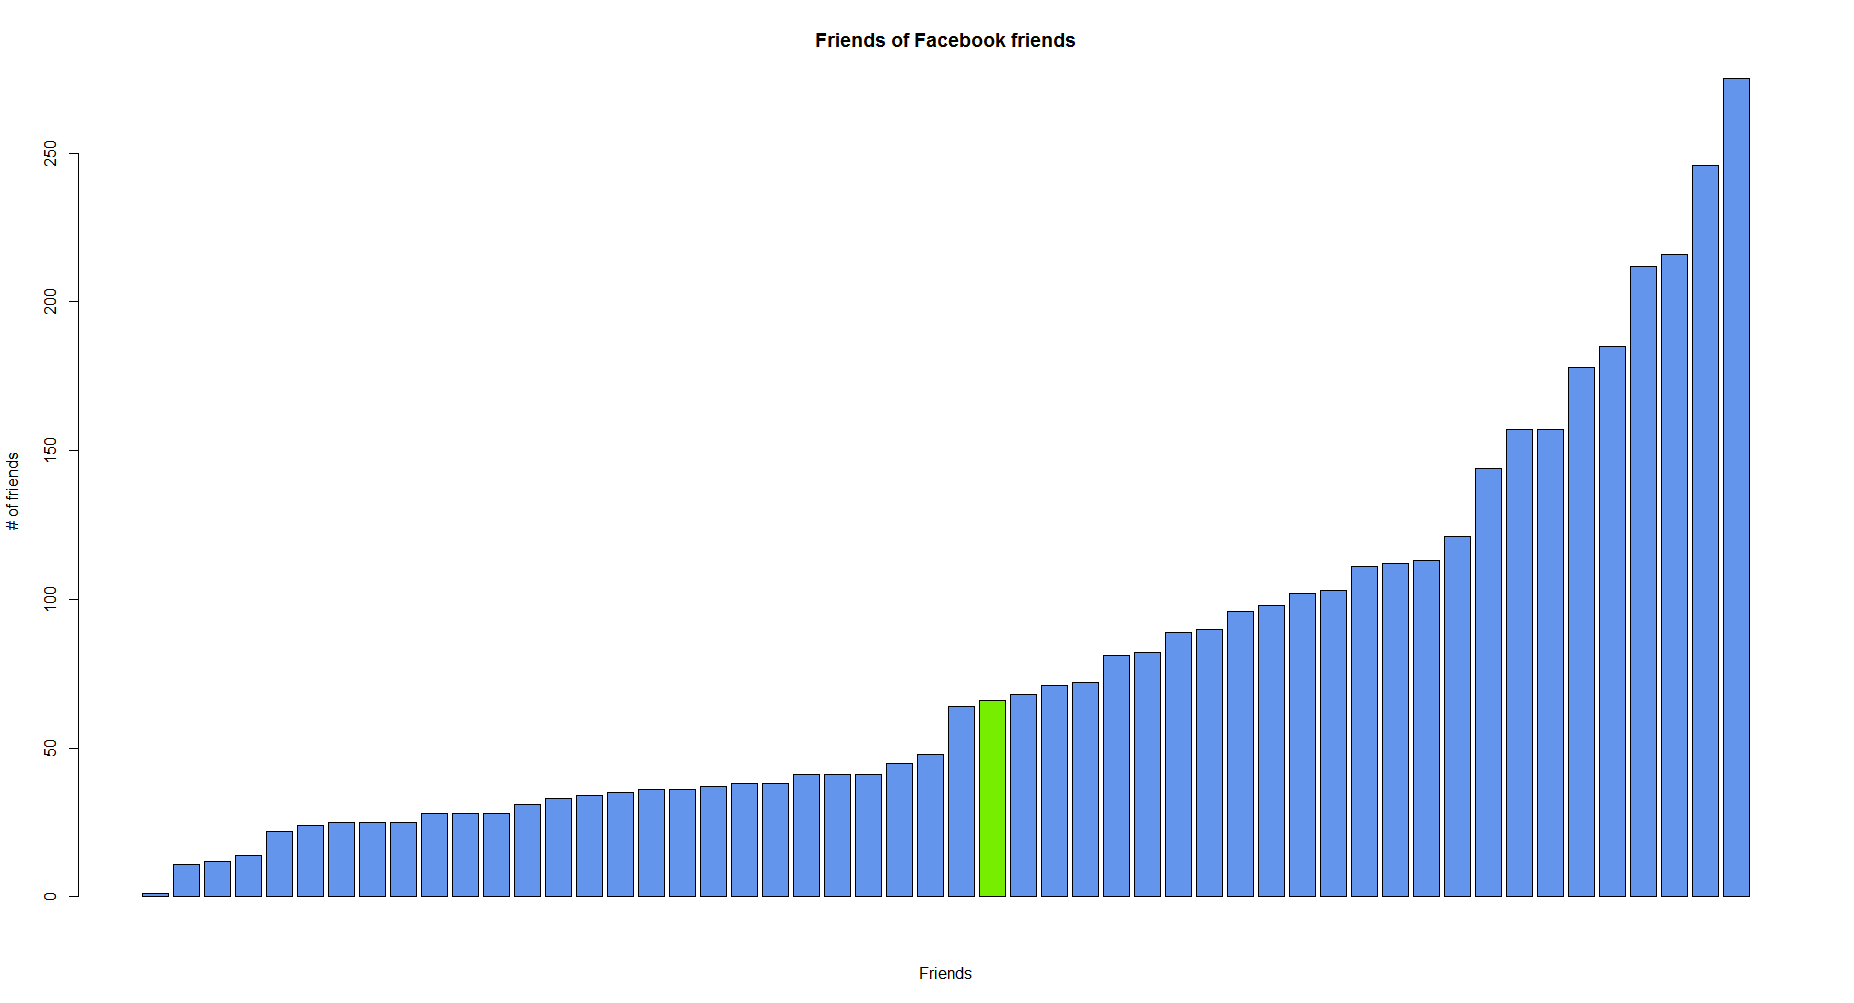
\includegraphics[width=0.8\textwidth]{Q3/1.png}
\caption{Initial View}
\label{fig:Initial View}
\end{figure}

\begin{figure}[!ht]
\centering
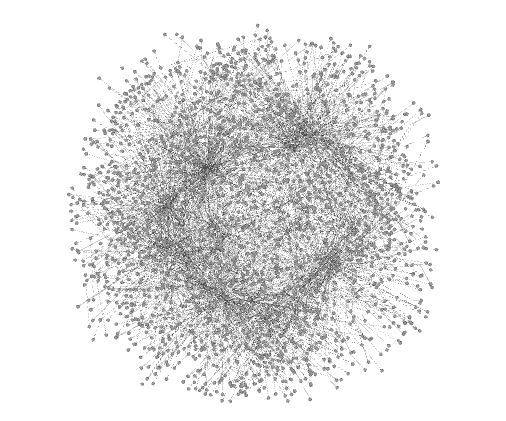
\includegraphics[width=0.8\textwidth]{Q3/2.png}
\caption{Using Yifan Hu' Layout}
\label{fig:Using Yifan Hu' Layout}
\end{figure}

\begin{figure}[!ht]
\centering
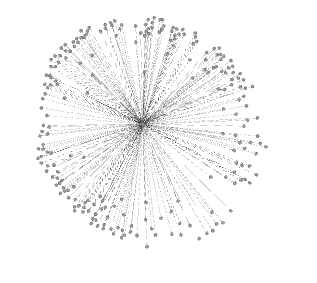
\includegraphics[width=0.8\textwidth]{Q3/4.png}
\caption{Using Filters}
\label{fig:Using Filters}
\end{figure}

\begin{figure}[!ht]
\centering
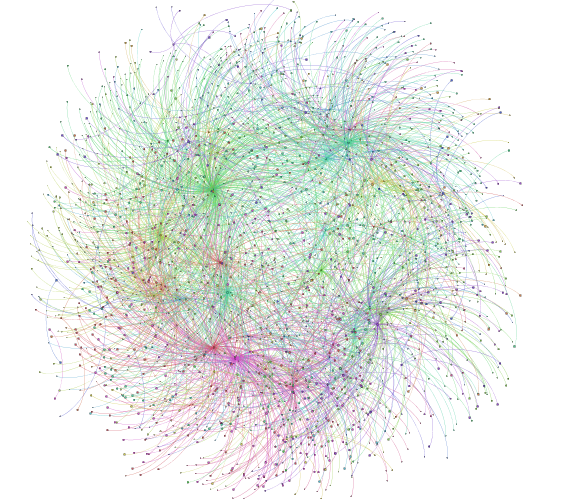
\includegraphics[width=0.8\textwidth]{Q3/3.png}
\caption{Color Nodes}
\label{fig:Color Nodes}
\end{figure}

\begin{figure}[!ht]
\centering
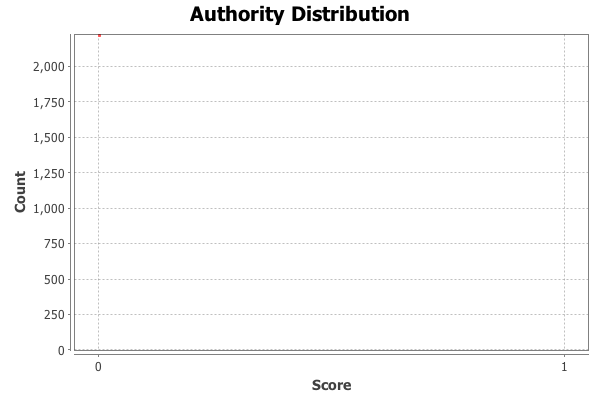
\includegraphics[width=0.8\textwidth]{Q3/Hits/authorities.png}
\caption{Hits Authorities}
\label{fig:Hits Authorities}
\end{figure}

\begin{figure}[!ht]
\centering
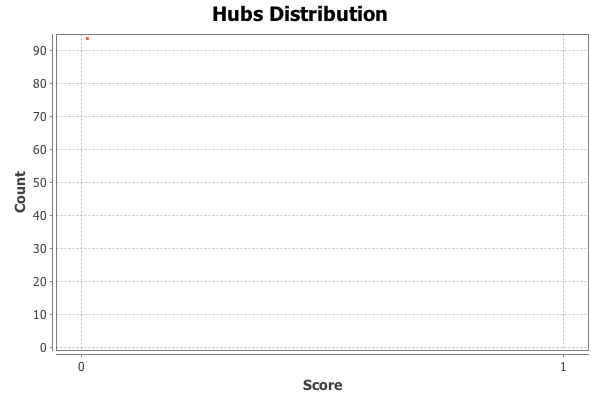
\includegraphics[width=0.8\textwidth]{Q3/Hits/hubs.png}
\caption{Hits Hubs}
\label{fig:Hits Hubs}
\end{figure}

\begin{figure}[!ht]
\centering
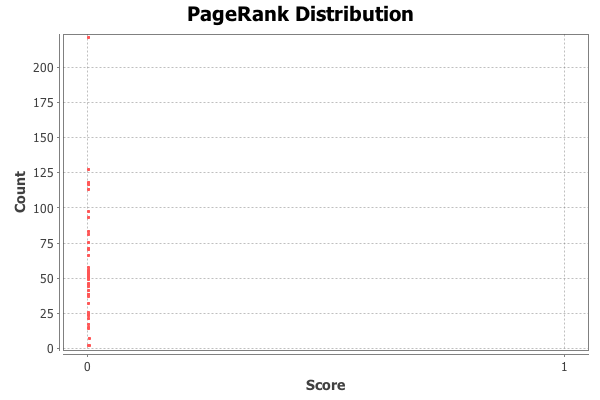
\includegraphics[width=0.8\textwidth]{Q3/PageRank/pageranks.png}
\caption{Page Ranks}
\label{fig:Page Ranks}
\end{figure}

\begin{figure}[!ht]
\centering
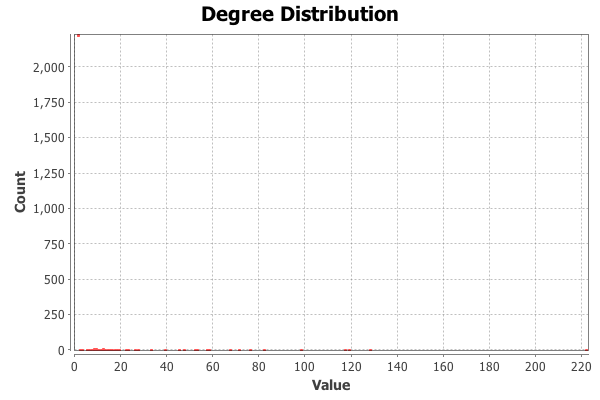
\includegraphics[width=0.8\textwidth]{Q3/AverageDegree/degree-distribution.png}
\caption{Average Degree: Degree Distribution}
\label{fig:Average Degree: Degree distribution}
\end{figure}

\begin{figure}[!ht]
\centering
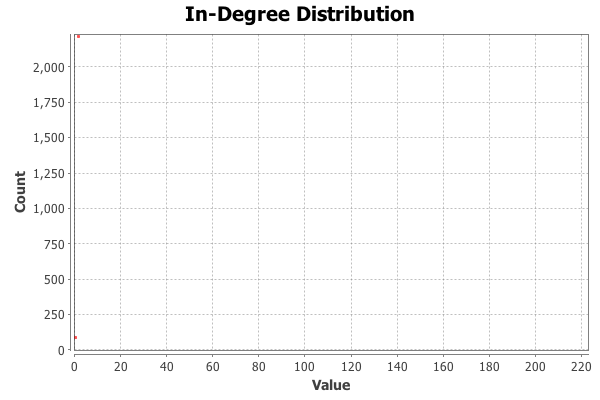
\includegraphics[width=0.8\textwidth]{Q3/AverageDegree/indegree-distribution.png}
\caption{Average Degree: Indegree Distribution}
\label{fig:Average Degree: Indegree distribution}
\end{figure}

\begin{figure}[!ht]
\centering
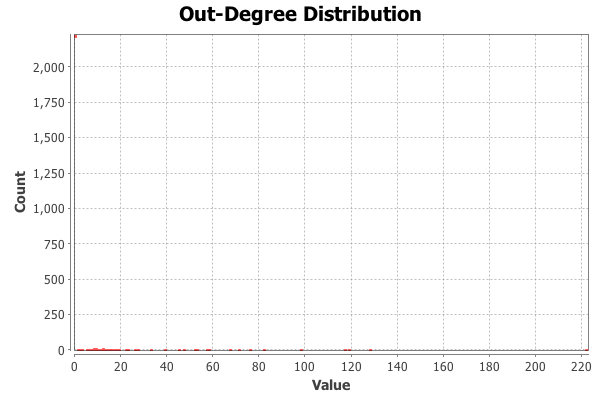
\includegraphics[width=0.8\textwidth]{Q3/AverageDegree/outdegree-distribution.png}
\caption{Average Degree: Outdegree Distribution}
\label{fig:Average Degree: Outdegree distribution}
\end{figure}

\begin{figure}[!ht]
\centering
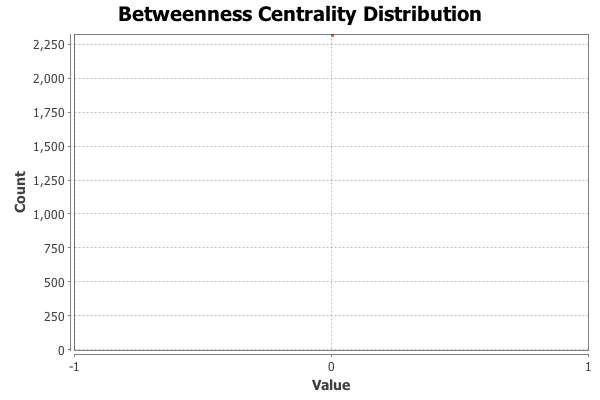
\includegraphics[width=0.8\textwidth]{Q3/NetworkDiameter/Betweenness Centrality Distribution.png}
\caption{Network Diameter: Betweenness Centrality Distribution}
\label{fig:Network Diameter Betweenness Centrality Distribution}
\end{figure}


\begin{figure}[!ht]
\centering
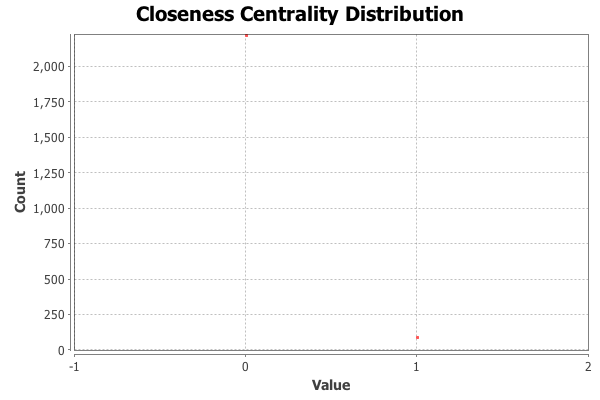
\includegraphics[width=0.8\textwidth]{Q3/NetworkDiameter/Closeness Centrality Distribution.png}
\caption{Network Diameter: Closeness Centrality Distribution}
\label{fig:Network Diameter Closeness Centrality Distribution}
\end{figure}

\begin{figure}[!ht]
\centering
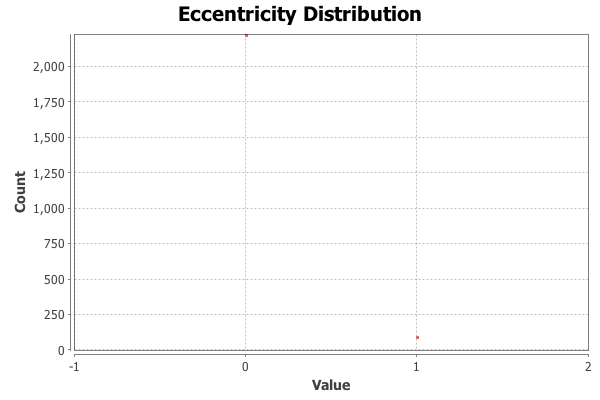
\includegraphics[width=0.8\textwidth]{Q3/NetworkDiameter/Eccentricity Distribution.png}
\caption{Network Diameter: Eccentricity Distribution}
\label{fig:Network Diameter Eccentricity Distribution}
\end{figure}

\begin{figure}[!ht]
\centering
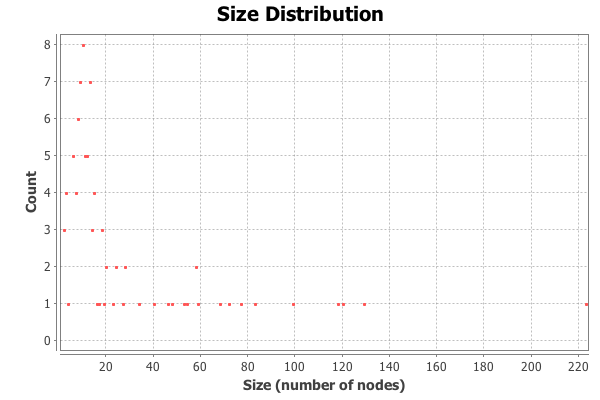
\includegraphics[width=0.8\textwidth]{Q3/NetworkDiameter/connectedcomponent/cc-size-distribution.png}
\caption{Network Diameter: Connected Component cc-size-distribution}
\label{fig:Network Diameter Connected Component cc-size-distribution}
\end{figure}

\end{document}